\documentclass{article}

% formato
\usepackage[margin = 1.5cm, letterpaper]{geometry}
\usepackage[utf8]{inputenc}

% autómatas
\usepackage{tikz}
\usetikzlibrary{automata, positioning}

%formato ecuaciones
\usepackage{amsmath}

% símbolos
\usepackage{amssymb}

% manejo de tablas
\usepackage{float}

\begin{document}
    \title{
        Autómatas y Lenguajes formales \\
        Ejercicio Semanal 6
    }

    \author{
        Sandra del Mar Soto Corderi \\
        Edgar Quiroz Castañeda
    }

    \date{
        14 de marzo del 2019
    }
    
    \maketitle

    \begin{enumerate}
        \item {
            Para cada 	$ANF_{\epsilon}$, resuelve los siguientes incisos.
            \begin{enumerate}
                \item Calcula la $\epsilon$-cerradura de cada estado.
                
				\item Elimina las $\epsilon$-transiciones obteniendo un AFN, 
				mostrando el proceso de cálculo de las nuevas transiciones.
            \end{enumerate}
        }
       \end{enumerate}
    	\begin{enumerate}
    		\item {
    			Autómata 1
    			\begin{figure} [H]
    				\centering
    				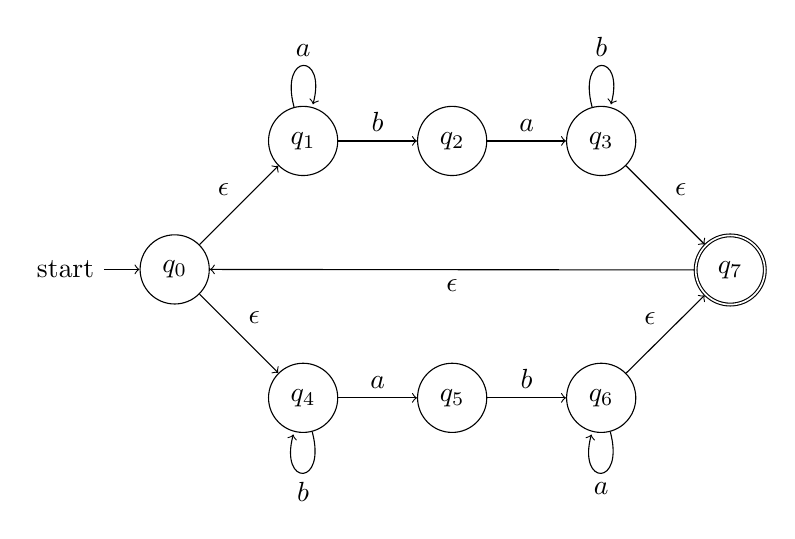
\begin{tikzpicture}[auto]
    				% estados
    				\node [state, initial] (q0) {$q_{0}$};
    				\node [state] (q1) [above right=of q0] {$q_{1}$};
    				\node [state] (q2) [right=of q1] {$q_{2}$};
    				\node [state] (q3) [right=of q2] {$q_{3}$};
    				\node [state] (q4) [below right=of q0] {$q_{4}$};
    				\node [state] (q5) [right=of q4] {$q_{5}$};
    				\node [state] (q6) [right=of q5] {$q_{6}$};
    				\node [state, accepting] (q7) [below right=of q3] {$q_{7}$};
    				
    				% transiciones
    				\path[->]
    				(q0) edge node {$\epsilon$} (q1)
    				(q0) edge node {$\epsilon$} (q4)
    				(q1) edge [loop above] node {$a$} (q1)
    				(q3) edge [loop above] node {$b$} (q3)
    				(q4) edge [loop below] node {$b$} (q4)
    				(q6) edge [loop below] node {$a$} (q6)
    				(q3) edge node {$\epsilon$} (q7)
    				(q6) edge node {$\epsilon$} (q7)
    				(q7) edge node {$\epsilon$} (q0)
    				(q1) edge node {$b$} (q2)
    				(q2) edge node {$a$} (q3)
    				(q4) edge node {$a$} (q5)
    				(q5) edge node {$b$} (q6);
    				\end{tikzpicture}
    			\end{figure}
    		}
    	\item {
    		Autómata 2
    		\begin{figure} [H]
    			\centering
    				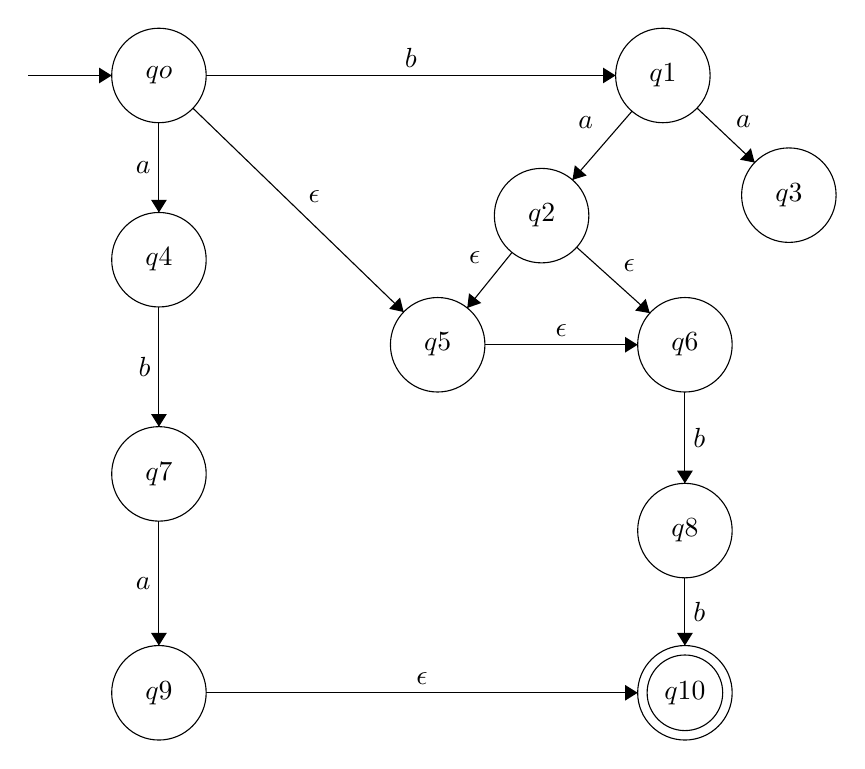
\begin{tikzpicture}[scale=0.2]
    				\tikzstyle{every node}+=[inner sep=0pt]
    				\draw [black] (12.3,-11.4) circle (3);
    				\draw (12.3,-11.4) node {$qo$};
    				\draw [black] (12.3,-23.1) circle (3);
    				\draw (12.3,-23.1) node {$q4$};
    				\draw [black] (12.3,-36.7) circle (3);
    				\draw (12.3,-36.7) node {$q7$};
    				\draw [black] (12.3,-50.6) circle (3);
    				\draw (12.3,-50.6) node {$q9$};
    				\draw [black] (44.3,-11.4) circle (3);
    				\draw (44.3,-11.4) node {$q1$};
    				\draw [black] (52.3,-19) circle (3);
    				\draw (52.3,-19) node {$q3$};
    				\draw [black] (36.6,-20.3) circle (3);
    				\draw (36.6,-20.3) node {$q2$};
    				\draw [black] (30,-28.5) circle (3);
    				\draw (30,-28.5) node {$q5$};
    				\draw [black] (45.7,-28.5) circle (3);
    				\draw (45.7,-28.5) node {$q6$};
    				\draw [black] (45.7,-40.3) circle (3);
    				\draw (45.7,-40.3) node {$q8$};
    				\draw [black] (45.7,-50.6) circle (3);
    				\draw (45.7,-50.6) node {$q10$};
    				\draw [black] (45.7,-50.6) circle (2.4);
    				\draw [black] (12.3,-39.7) -- (12.3,-47.6);
    				\fill [black] (12.3,-47.6) -- (12.8,-46.8) -- (11.8,-46.8);
    				\draw (11.8,-43.65) node [left] {$a$};
    				\draw [black] (34.72,-22.64) -- (31.88,-26.16);
    				\fill [black] (31.88,-26.16) -- (32.77,-25.85) -- (31.99,-25.23);
    				\draw (32.74,-22.97) node [left] {$\epsilon$};
    				\draw [black] (42.34,-13.67) -- (38.56,-18.03);
    				\fill [black] (38.56,-18.03) -- (39.46,-17.75) -- (38.71,-17.1);
    				\draw (39.9,-14.4) node [left] {$a$};
    				\draw [black] (46.47,-13.47) -- (50.13,-16.93);
    				\fill [black] (50.13,-16.93) -- (49.89,-16.02) -- (49.2,-16.75);
    				\draw (49.42,-14.72) node [above] {$a$};
    				\draw [black] (33,-28.5) -- (42.7,-28.5);
    				\fill [black] (42.7,-28.5) -- (41.9,-28) -- (41.9,-29);
    				\draw (37.85,-28) node [above] {$\epsilon$};
    				\draw [black] (38.83,-22.31) -- (43.47,-26.49);
    				\fill [black] (43.47,-26.49) -- (43.21,-25.58) -- (42.54,-26.33);
    				\draw (42.16,-23.91) node [above] {$\epsilon$};
    				\draw [black] (15.3,-50.6) -- (42.7,-50.6);
    				\fill [black] (42.7,-50.6) -- (41.9,-50.1) -- (41.9,-51.1);
    				\draw (29,-50.1) node [above] {$\epsilon$};
    				\draw [black] (4,-11.4) -- (9.3,-11.4);
    				\fill [black] (9.3,-11.4) -- (8.5,-10.9) -- (8.5,-11.9);
    				\draw [black] (45.7,-31.5) -- (45.7,-37.3);
    				\fill [black] (45.7,-37.3) -- (46.2,-36.5) -- (45.2,-36.5);
    				\draw (46.2,-34.4) node [right] {$b$};
    				\draw [black] (15.3,-11.4) -- (41.3,-11.4);
    				\fill [black] (41.3,-11.4) -- (40.5,-10.9) -- (40.5,-11.9);
    				\draw (28.3,-10.9) node [above] {$b$};
    				\draw [black] (12.3,-26.1) -- (12.3,-33.7);
    				\fill [black] (12.3,-33.7) -- (12.8,-32.9) -- (11.8,-32.9);
    				\draw (11.8,-29.9) node [left] {$b$};
    				\draw [black] (14.46,-13.48) -- (27.84,-26.42);
    				\fill [black] (27.84,-26.42) -- (27.61,-25.5) -- (26.92,-26.22);
    				\draw (22.17,-19.47) node [above] {$\epsilon$};
    				\draw [black] (12.3,-14.4) -- (12.3,-20.1);
    				\fill [black] (12.3,-20.1) -- (12.8,-19.3) -- (11.8,-19.3);
    				\draw (11.8,-17.25) node [left] {$a$};
    				\draw [black] (45.7,-43.3) -- (45.7,-47.6);
    				\fill [black] (45.7,-47.6) -- (46.2,-46.8) -- (45.2,-46.8);
    				\draw (46.2,-45.45) node [right] {$b$};
    				\end{tikzpicture}
    		\end{figure}
    		\begin{enumerate}
    			\item {
    				Calcula la $\epsilon$-cerradura de cada estado
    				\begin{align*}
    					Cl_{\epsilon}(q_{0}) &= \{q_{0}, q_{5}, q_{6}\}
    					&Cl_{\epsilon}(q_{1}) &= \{q_{1}\} \\
    					Cl_{\epsilon}(q_{2}) &= \{q_{2}, q_{5}, q_{6}\}
    					&Cl_{\epsilon}(q_{3}) &= \{q_{3}\} \\
    					Cl_{\epsilon}(q_{4}) &= \{q_{4}\}
    					&Cl_{\epsilon}(q_{5}) &= \{q_{5}, q_{6}\} \\
    					Cl_{\epsilon}(q_{6}) &= \{q_{6}\}
    					&Cl_{\epsilon}(q_{7}) &= \{q_{7}\} \\
    					Cl_{\epsilon}(q_{8}) &= \{q_{8}\}
    					&Cl_{\epsilon}(q_{9}) &= \{q_{9}, q_{10}\} \\
    					Cl_{\epsilon}(q_{10}) &= \{q_{10}\} 
    				\end{align*}
				}
				\item {
					Elimina las $\epsilon$-transiciones obteniendo un AFN, 
					mostrando el proceso de cálculo de las nuevas transiciones.\\
					Sea $M_{\epsilon} = \langle Q_{\epsilon}, \Sigma_{\epsilon},
					 \delta_{\epsilon}, q_{0\epsilon}, F_{\epsilon} \rangle$ el atómata de la figura.\\
					El nuevo automata sería $M = \langle Q, \Sigma, \delta, 
					q_{0}, F \rangle$ dado por 
					\[\ Q = Q_{\epsilon},\ \Sigma = \Sigma_{\epsilon},
					\ q_0 = q_{0\epsilon},\ F = F_{\epsilon}\]
					Pues $F_{\epsilon} \cap Cl_{\epsilon}(q_{0}) = \varnothing$.\\
					En cuento a la $\delta$, esta se construye de la siguiente 
					manera
					\begin{align*}
						\delta(q_{0}, a) &= \delta^{*}_{\epsilon}(q_{0}, a) \\
						&= Cl_{\epsilon}(\bigcup_{p \in \delta_{\epsilon}(q_{0}, \epsilon)}
						{\delta_{\epsilon}(p, a)}) \\
						&= Cl_{\epsilon}(\delta_{\epsilon}(q_{0}, a) 
						\cup \delta_{\epsilon}(q_{5}, a)
						\cup \delta_{\epsilon}(q_{6}, a))\\
						&= Cl_{\epsilon}(\{q_{4}\} \cup \varnothing \cup \varnothing)\\
						&= \{q_{4}\}
					\end{align*}

					\begin{align*}
						\delta(q_{0}, b) &= \delta^{*}_{\epsilon}(q_{0}, b) \\
						&= Cl_{\epsilon}(\bigcup_{p \in \delta_{\epsilon}(q_{0}, \epsilon)}
						{\delta_{\epsilon}(p, b)}) \\
						&= Cl_{\epsilon}(\delta_{\epsilon}(q_{0}, b) 
						\cup \delta_{\epsilon}(q_{5}, b)
						\cup \delta_{\epsilon}(q_{6}, b))\\
						&= Cl_{\epsilon}(\{q_{1}\} \cup \varnothing \cup \{q_{8}\})\\
						&= \{q_{1}, q_{8}\}
					\end{align*}

					\begin{align*}
						\delta(q_{1}, a) &= \delta^{*}_{\epsilon}(q_{1}, a) \\
						&= Cl_{\epsilon}(\bigcup_{p \in \delta_{\epsilon}(q_{1}, \epsilon)}
						{\delta_{\epsilon}(p, a)}) \\
						&= Cl_{\epsilon}(\delta_{\epsilon}(q_{1}, a))\\
						&= Cl_{\epsilon}(\{q_{2}, q_{3}\})\\
						&= \{q_{2}, q_{3}, q_{5}, q_{6}\}
					\end{align*}

					\begin{align*}
						\delta(q_{1}, b) &= \delta^{*}_{\epsilon}(q_{1}, b) \\
						&= Cl_{\epsilon}(\bigcup_{p \in \delta_{\epsilon}(q_{1}, \epsilon)}
						{\delta_{\epsilon}(p, b)}) \\
						&= Cl_{\epsilon}(\delta_{\epsilon}(q_{1}, b)) \\
						&= Cl_{\epsilon}(\varnothing) \\
						&= \varnothing
					\end{align*}

					\begin{align*}
						\delta(q_{2}, a) &= \delta^{*}_{\epsilon}(q_{2}, a) \\
						&= Cl_{\epsilon}(\bigcup_{p \in \delta_{\epsilon}(q_{2}, \epsilon)}
						{\delta_{\epsilon}(p, a)}) \\
						&= Cl_{\epsilon}(\delta_{\epsilon}(q_{2}, a) 
						\cup \delta_{\epsilon}(q_{5}, a)
						\cup \delta_{\epsilon}(q_{6}, a))\\
						&= Cl_{\epsilon}(\varnothing \cup \varnothing \cup \varnothing)\\
						&= \varnothing
					\end{align*}

					\begin{align*}
						\delta(q_{2}, b) &= \delta^{*}_{\epsilon}(q_{2}, b) \\
						&= Cl_{\epsilon}(\bigcup_{p \in \delta_{\epsilon}(q_{2}, \epsilon)}
						{\delta_{\epsilon}(p, b)}) \\
						&= Cl_{\epsilon}(\delta_{\epsilon}(q_{2}, b) 
						\cup \delta_{\epsilon}(q_{5}, b)
						\cup \delta_{\epsilon}(q_{6}, b))\\
						&= Cl_{\epsilon}(\varnothing \cup \varnothing \cup \{q_{8}\})\\
						&= \{q_{8}\}
					\end{align*}

					\begin{align*}
						\delta(q_{3}, a) &= \delta^{*}_{\epsilon}(q_{3}, a) \\
						&= Cl_{\epsilon}(\bigcup_{p \in \delta_{\epsilon}(q_{3}, \epsilon)}
						{\delta_{\epsilon}(p, a)}) \\
						&= Cl_{\epsilon}(\delta_{\epsilon}(q_{3}, a))\\
						&= Cl_{\epsilon}(\varnothing)\\
						&= \varnothing
					\end{align*}

					\begin{align*}
						\delta(q_{3}, b) &= \delta^{*}_{\epsilon}(q_{3}, b) \\
						&= Cl_{\epsilon}(\bigcup_{p \in \delta_{\epsilon}(q_{3}, \epsilon)}
						{\delta_{\epsilon}(p, b)}) \\
						&= Cl_{\epsilon}(\delta_{\epsilon}(q_{3}, b))\\
						&= Cl_{\epsilon}(\varnothing)\\
						&= \varnothing
					\end{align*}

					\begin{align*}
						\delta(q_{4}, a) &= \delta^{*}_{\epsilon}(q_{4}, a) \\
						&= Cl_{\epsilon}(\bigcup_{p \in \delta_{\epsilon}(q_{4}, \epsilon)}
						{\delta_{\epsilon}(p, a)}) \\
						&= Cl_{\epsilon}(\delta_{\epsilon}(q_{4}, a) 
						\cup \delta_{\epsilon}(q_{5}, a)
						\cup \delta_{\epsilon}(q_{6}, a))\\
						&= Cl_{\epsilon}(\{q_{4}\} \cup \varnothing \cup \varnothing)\\
						&= \{q_{4}\}
					\end{align*}

					\begin{align*}
						\delta(q_{4}, b) &= \delta^{*}_{\epsilon}(q_{4}, b) \\
						&= Cl_{\epsilon}(\bigcup_{p \in \delta_{\epsilon}(q_{4}, \epsilon)}
						{\delta_{\epsilon}(p, b)}) \\
						&= Cl_{\epsilon}(\delta_{\epsilon}(q_{4}, b) 
						\cup \delta_{\epsilon}(q_{5}, b)
						\cup \delta_{\epsilon}(q_{6}, b))\\
						&= Cl_{\epsilon}(\{q_{1}\} \cup \varnothing \cup \{q_{8}\})\\
						&= \{q_{1}, q_{8}\}
					\end{align*}

				}
    		\end{enumerate}
    	}
    \end{enumerate}
\end{document}